\chapter{Arithmetic admissibility in SELECT-II}\label{ch:arith}

Which orderings of a set of labels can SELECT-II produce from a given source? This chapter shows that the answer is governed by a single law, the \emph{prefix law}: admissibility is decided by the denominators of products over prefix sets. Everything topological in the later chapters is built on it. Throughout, a \emph{content} is a set $C=\{c_0<\dots<c_{k-1}\}$ of distinct positive integers, a label is addressed by its \emph{rank} $r\in\{0,\dots,k-1\}$, an arrangement is a permutation of the ranks, and $A_C(m)\subseteq S_k$ is the set of arrangements admissible from the source $m$ (\cref{sec:complex}).

\section{The prefix law}
For a set $I$ of ranks put $R(I)=\prod_{r\in I}\frac{(c_r+1)^2}{c_r}\in\Q$ (with $R(\emptyset)=1$) and let $D(I)$ be the denominator of $R(I)$ in lowest terms. For an arrangement $w=(w_1,\dots,w_k)$ with prefix sets $I_j=\{w_1,\dots,w_j\}$ define its \emph{threshold} $K(w)=\operatorname{lcm}_{1\le j\le k}D(I_j)$.

@@lem:F@@

Hence arithmetic admissibility is \emph{prefix-defined} in the sense of \cref{def:prefix-defined}, with the family $\mathfrak F_C(m)=\{I: D(I)\mid m\}$. (The last prefix set is $[k]$ itself; if $D([k])\nmid m$ then $A_C(m)$ is empty, and for nonempty $A_C(m)$ the condition at $[k]$ is automatic.) Everything in \cref{ch:swaps,ch:topology,ch:duality} that holds for prefix-defined sets therefore applies to SELECT-II.

The law becomes concrete in terms of $p$-adic valuations.
@@prop:valuation@@
A label contributes a positive weight at $p$ when $p\mid c_r$ (it \emph{consumes} $p$-divisibility of the state) and a negative weight $-2v_p(c_r+1)$ when $p\mid c_r+1$ (it \emph{supplies} it). Only primes dividing some $c_r$ or $c_r+1$ matter. \Cref{fig:thresholds} shows these weights for the anchor content $\lambda_A=(2,3,4,5,8,9)$ together with the valuations the source must reach for the prefix sets that will matter in \cref{ch:topology}.

\begin{figure}[ht]\centering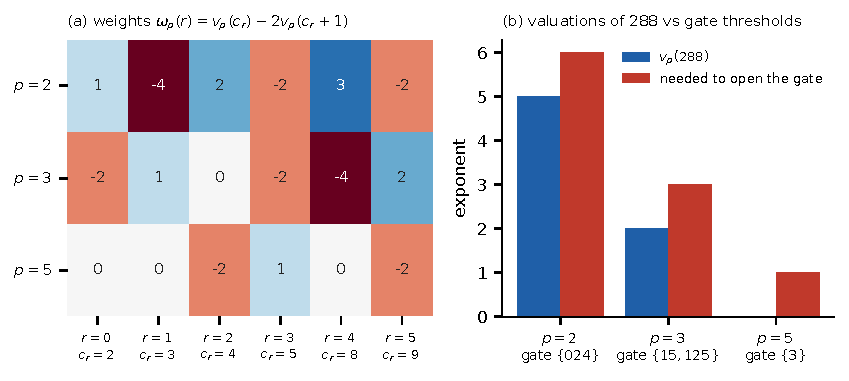
\includegraphics[width=\textwidth]{figures/fig_thresholds.pdf}
\caption{Arithmetic of admissibility for $\lambda_A=(2,3,4,5,8,9)$. (a) The weights $\omega_p(r)=v_p(c_r)-2v_p(c_r+1)$: positive entries (blue) consume divisibility, negative entries (red) supply it. (b) For the three primes $2,3,5$: the valuation of $m=288=2^5\cdot3^2$ (bars) against the valuation a prefix set needs. The cycle's own prefix sets are all admissible at $288$; each of the three \emph{gates} $\{024\}$, $\{15,125\}$, $\{3\}$ needs exactly one more power of $2$, $3$ or $5$ (\cref{ch:topology}).}\label{fig:thresholds}
\end{figure}

@@prop:finite-lattice@@
For the content $\lambda_A=(2,3,4,5,8,9)$ the caps are $2^6,3^3,5^1$, giving $56$ systems, and for $\lambda_B=(2,3,6,7,8,9)$ they are $2^5,3^4,7^1$ (and $0$ at $5$), giving $60$. These are the two \emph{anchor contents} of \cref{ch:topology}. The source line collapses to a finite lattice of regimes: for example the sixty sources $288t$ realise only eight distinct regimes for either anchor.

\section{Closure and minimal sources}
Define for $S\subseteq S_k$ the \emph{lcm} $L(S)=\operatorname{lcm}_{w\in S}K(w)$, with $L(\emptyset)=1$, and the \emph{closure} $\cl_K(S)=\{v\in S_k:\ K(v)\mid L(S)\}$. Call $S$ \emph{realizable} if $S=A_C(m)$ for some $m$. The family $\mathcal A(C)=\{A_C(m):m\in\N\}$ includes $\emptyset$ when some $A_C(m)$ is empty.

@@thm:closure@@
@@ex:erratum@@

\section{Block factorization and the cube-product property}
@@thm:block@@
@@cor:CP@@

\section{Face thresholds and the divisibility filtration}
@@thm:face-threshold@@
The complexes $X_C(m)=K_{A_C(m)}$ thus form a multi-parameter filtration indexed by the exponent vectors $(v_q(m))_q$: the \emph{source filtration at fixed content}, not the evolution of a state under SELECT-II. The events of this filtration, a face being born as $m$ becomes more divisible, are the arithmetic activations studied in \cref{ch:topology}.

\section{Counting laws on the anchors}
The regime sizes $N(m)=|A_C(m)|$ are the simplest observable of the filtration. For $\lambda_A$ at $m=288t$ the eight regimes with $A_C(288)\subseteq A_C(288t)$ have sizes $372,408,444,480,612,648,684,720$, and for $\lambda_B$ at $m=432t$ sizes $276,312,324,360,612,648,684,720$.
@@obs:counting+finite-exact@@
These laws are used in \cref{ch:separation}: on the comparable window the count $N$ is injective in the regime, which is why $N$ alone recovers the hole state there.
